



\begin{frame}[c]{Resumo do Conteúdo Programático}
	\vspace{1mm}
%	\centering
\begin{multicols}{2}

	\makebox[0.5\textwidth][c]{       %centering table
		\scalebox{0.6}{
			{\renewcommand{\arraystretch}{1.3}
				\fontsize{9pt}{13}\selectfont{
					\pgfplotstabletypeset[col sep=&,
					string type,
					column type=l,
					% columns/Nome Completo/.style={column name={Nome Completo}, column  type={l}},
					columns/0/.style={column name=N,column type={|l|}},
					columns/1/.style={column name=Aulas, column type={l}},
					columns/2/.style={column name=Mês, column type={|l}},
					columns/3/.style={column name=Data, column type={|l}},
					columns/4/.style={column name={Conteúdo Previsto}, column type={|l}},
					every head row/.style={before row=\hline,after row=\hline},
					every last row/.style={after row=\hline},
					after row={\hline},
					every head row/.style={
						before row={
							\noalign{\hrule height 1.5pt}
						},
						after row={
							\hline
						},  
					},
					every last row/.style={
						after row=\noalign{\hrule height 1.5pt}
					},
					col sep = comma,
					every head row/.style={
						before row={\hline\rowcolor{yellow!25}},after row=\hline
					},
					every row no 1/.style={
						before row={\rowcolor{green!25}}
					},
					every row no 3/.style={
						before row={\rowcolor{green!25}}
					},
					every row no 5/.style={
						before row={\rowcolor{green!25}}
					},
					every row no 7/.style={
						before row={\rowcolor{green!25}}
					},
					every row no 9/.style={
						before row={\rowcolor{green!25}}
					},
					every row no 11/.style={
						before row={\rowcolor{green!25}}
					},
					every row no 13/.style={
						before row={\rowcolor{green!25}}
					},
					every row no 15/.style={
						before row={\rowcolor{green!25}}
					},
					every row no 17/.style={
						before row={\rowcolor{green!25}}
					},
					every row no 19/.style={
						before row={\rowcolor{green!25}}
					},
					every row no 21/.style={
						before row={\rowcolor{green!25}}
					},
					every row no 22/.style={
						before row={\rowcolor{red!25}}
					},
				 	every row no 24/.style={
				 		before row={\rowcolor{green!25}}
				 	},
				    every row no 26/.style={
				        before row={\rowcolor{green!25}}
				    },
					every row no 28/.style={
						before row={\rowcolor{green!25}}
					},
					every row no 30/.style={
						before row={\rowcolor{green!25}}
					},
					every row no 31/.style={
						before row={\rowcolor{green!25}}
					},
					every row no 33/.style={
						before row={\rowcolor{green!25}}
					},
					every row no 35/.style={
						before row={\rowcolor{green!25}}
					},
				% 	every row no 20/.style={
				% 		before row={\rowcolor{green!25}}
				% 	},
					skip rows between index={30}{77},
					]{\cronograma}
		}}}
	}
	

\columnbreak


	\makebox[0.5\textwidth][c]{       %centering table
	\scalebox{0.55}{
		{\renewcommand{\arraystretch}{1.3}
			\fontsize{9pt}{13}\selectfont{
				\pgfplotstabletypeset[col sep=&,
				string type,
				column type=l,
				% columns/Nome Completo/.style={column name={Nome Completo}, column  type={l}},
				columns/0/.style={column name=N,column type={|l|}},
				columns/1/.style={column name=Aulas, column type={l}},
				columns/2/.style={column name=Mês, column type={|l}},
				columns/3/.style={column name=Data, column type={|l}},
				columns/4/.style={column name={Conteúdo Previsto}, column type={|l}},
				every head row/.style={before row=\hline,after row=\hline},
				every last row/.style={after row=\hline},
				after row={\hline},
				every head row/.style={
					before row={
						\noalign{\hrule height 1.5pt}
					},
					after row={
						\hline
					},  
				},
				every last row/.style={
					after row=\noalign{\hrule height 1.5pt}
				},
				col sep = comma,
				every head row/.style={
					before row={\hline\rowcolor{yellow!25}},after row=\hline
				},
				every row no 1/.style={
					before row={\rowcolor{green!25}}
				},
				every row no 3/.style={
					before row={\rowcolor{green!25}}
				},
				every row no 5/.style={
					before row={\rowcolor{red!25}}
				},
				every row no 7/.style={
					before row={\rowcolor{green!25}}
				},
				every row no 9/.style={
					before row={\rowcolor{green!25}}
				},
				every row no 11/.style={
					before row={\rowcolor{green!25}}
				},
				every row no 13/.style={
					before row={\rowcolor{green!25}}
				},
				every row no 15/.style={
					before row={\rowcolor{green!25}}
				},
				every row no 16/.style={
					before row={\rowcolor{red!25}}
				},
				every row no 19/.style={
					before row={\rowcolor{green!25}}
				},
				every row no 21/.style={
					before row={\rowcolor{red!25}}
				},
				every row no 23/.style={
					before row={\rowcolor{green!25}}
				},
				every row no 25/.style={
					before row={\rowcolor{green!25}}
				},
				every row no 27/.style={
					before row={\rowcolor{green!25}}
				},
				every row no 29/.style={
					before row={\rowcolor{green!25}}
				},
				every row no 30/.style={
					before row={\rowcolor{green!25}}
				},
				every row no 31/.style={
					before row={\rowcolor{green!25}}
				},
				every row no 33/.style={
					before row={\rowcolor{green!25}}
				},
				every row no 35/.style={
					before row={\rowcolor{green!25}}
				},
				% 	every row no 20/.style={
					% 		before row={\rowcolor{green!25}}
					% 	},
				skip rows between index={0}{36},
				]{\cronograma}
	}}}
}



\end{multicols}
	
\end{frame}




\begin{frame}[t]{Quem sou eu?}

    \begin{columns}[onlytextwidth,T]
		\column{\dimexpr\linewidth-30mm}
		\vspace{1em}
		
		Prof. Dr. Bruno Iran Ferreira Maciel, 41
    
        \vspace{2mm}
        Atuo como professor; desenvolvedor; e consultor de TI.
        
        \vspace{4mm}
    
      \fontsize{10pt}{12}\selectfont{
    	\begin{itemize}%[<+->]  
    	    \item Doutor em Ciência da Computação, 2015-2020
%    	    \item Técnico em Análise e Desenvolvimento de Software, 2017-2018
    	    \item Mestre em Ciência da Computação, 2012-2014
    	    \item Especialista em Engenharia e Reúso de Software, 2011-2012
    	    \item Graduado em Sistemas de Informação, 2016-2016
    	    \item Graduado em Ciência da Computação, 2007-2011
    	    \item Técnico em Análise e Desenvolvimento de Software, 2007-2007
    	    \item CV completo \url{http://bit.ly/brunomaciel-lattes}
    	\end{itemize}
    	}\par
		
		\column{30mm}
		\centering
		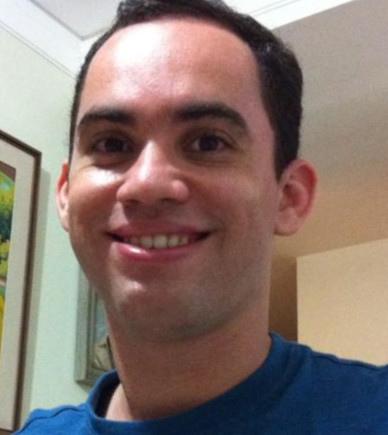
\includegraphics[scale=0.15]{imagens/prof-bruno.jpg}
		
	\end{columns}
	
	
% % 	\begin{minipage}[r]{.15\textwidth}
% % % 	\vspace{1cm}
% %     \end{minipage}
%     \hfill\begin{flushright}% or better \raggedleft see comments below
%   \vspace{-1em}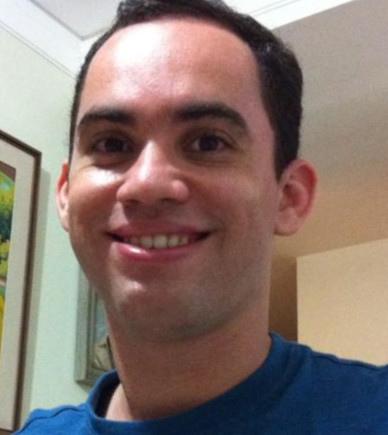
\includegraphics[scale=0.15]{imagens/prof-bruno.jpg}
%  \end{flushright}

    
%     \begin{minipage}{.85\textwidth}
%     Prof. Dr. Bruno Iran Ferreira Maciel, 37
    
%     \vspace{2mm}
%     Atualmente atuo como professor de ensino superior; Engenheiro de sistemas; e consultor de TI.
    
%     \vspace{2mm}
    
%       \fontsize{10pt}{12}\selectfont{
%     	\begin{itemize}%[<+->]  
%     	    \item Doutor em Ciência da Computação, 2015-2020
%     	    \item Mestre em Ciência da Computação, 2012-2014
%     	    \item Especialista em Engenharia e Reúso de Software, 2011-2012
%     	    \item Graduado em Sistemas de Informação, 2016-2016
%     	    \item Graduado em Ciência da Computação, 2007-2011
%     	    \item Técnico em Análise e Desenvolvimento de Software, 2007-2007
%     	    \item CV completo \url{http://bit.ly/brunomaciel-lattes}
%     	\end{itemize}
%     	}\par
%     \end{minipage}

% 	\vspace{1em}
% 	\centering
% \fontsize{20pt}{15.2}\selectfont{
% E-mail:	esuda@brunomaciel.com
% 	\vspace{1em}
% 	}\par
	
\end{frame}


\begin{frame}{}
    \fontsize{14pt}{15.2}\selectfont{
	Apresentação pessoal, integração com a turma, introdução de conceitos básicos de desenvolvimento de softwae e despertar curiosidade dos alunos sobre o tema.
	
	\vspace{1em}
	}\par
	\vspace{1em}
\end{frame}


\begin{frame}{Compromisso semanal}
%     \fontsize{14pt}{15.2}\selectfont{
% 	Datas importantes
% 	\vspace{1em}
% 	}\par
	
	\fontsize{9pt}{12}\selectfont{
	Encontros: sextas e sábados
	\begin{itemize}%[<+->]  
	    \item Período: 02/08/2024 à 30/11/2024
	    
	   % \item Laboratório: 4
	\end{itemize}
	
	\vspace{0.5em}
	Sextas
	\begin{itemize}%[<+->]  
		\item Início: 18h
		\item Térmico: 21h - Sem intervalo
		\item Térmico: 21h10 - Com intervalo de 10 minutos (a confirmar)
	\end{itemize}
	
	\vspace{0.5em}
	Sábados
	\begin{itemize}%[<+->]  

		\item Início: 9h
		\item Térmico: 12h - Sem intervalo
		\item Térmico: 12h10 - Com intervalo de 10 minutos (a confirmar)
	\end{itemize}
	
	\vspace{0.5em}
	Reposições de aulas aos Sábados no período da tarde
	\begin{itemize}%[<+->] 		
		\item Início: 14h
		\item Térmico: 17h - Sem intervalo
		\item Térmico: 17h10 - Com intervalo de 10 minutos (a confirmar)
	\end{itemize}
	
	}\par
	
	\vspace{1em}
\end{frame}


\begin{frame}{Metodologia das Aulas}
Aulas:

    \fontsize{10pt}{12}\selectfont{
    \begin{itemize}%[<+->]  
        \item 18h-19h30
        \item 19h30-21h
	\end{itemize}
	}\par
	\vspace{0.5em}
	\fontsize{12pt}{15}\selectfont{
		\begin{itemize}%[<+->]  
	    \item Resolução de dúvidas gerais e tolerância: 18h até 18h15 (15 minutos)
	    \item Revisão da aula passada: 18h15 até 18h30 (15 minutos)
	    \item Adição de novo conteúdo: 18h30 até 21h (2h30)
	   % \item Exercício em sala de aula: 21h até 21h20m (20min)
	   % \item Revisão/dúvidas do novo conteúdo: 21h20m até 21h30m (10m)
	\end{itemize}
	}\par
	\vspace{1em}
\end{frame}

%\begin{frame}{Metodologia das Avaliação}
%
%	\fontsize{12pt}{15}\selectfont{
%	\begin{itemize}%[<+->]  
%	    \item Primeira nota: (exercício + prova)
%	        \begin{itemize}%[<+->]  
%        	    \item Exercícios (peso +1)
%        	    \item Prova escrita (peso 10)
%        	\end{itemize}
%    	\item Segunda nota: (exercício + prova + seminário)
%	        \begin{itemize}%[<+->]  
%        	    \item Exercícios (peso +1)
%        	    \item Prova escrita (peso 7)
%        	    \item Seminário (peso 3)
%        	\end{itemize}
%	\end{itemize}
%	}\par
%	\vspace{1em}
%\end{frame}

%\begin{frame}{Avisos}
%
%	\fontsize{12pt}{15}\selectfont{
%	\begin{itemize}%[<+->]  
%	    \item Frequência escolar:
%	        \begin{itemize}%[<+->]  
%        	    \item Número de faltas maior que 25\% = |Reprovado por faltas|
%        	    \item Cada dia de aula faltado equivale à 4 faltas;
%        	    \item Há 15 dias de aulas no cronograma |15 = 100\%|;
%        	    \item 4 dias faltados equivale a $\pm$ 26\%.
%         	\end{itemize}
%    	\item Atraso na entrega de atividade:
%	        \begin{itemize}%[<+->]  
%        	    \item Cada dia atrasado tem penalidade de menos 10\% do peso.
%        	    \item Tempo máximo de atraso tolerado = 7 dias.
%        	\end{itemize}
%	\end{itemize}
%	}\par
%	\vspace{1em}
%\end{frame}



\begin{frame}[t]{EMENTA}
\vspace{1cm}
	\fontsize{12pt}{16}\selectfont{
	O curso tem como objetivo desenvolver as habilidades necessárias em programação, noções de padrões de desenvolvimento de software, arquitetura cliente-servidor, noções de banco de dados e frameworks back-end para que você seja capaz de projetar soluções web que sejam seguras, robustas e escaláveis, com base em tecnologias modernas e nas melhores práticas de desenvolvimento de software.
	}\par
	\vspace{1em}
\end{frame}

\begin{frame}[t]{OBJETIVO}
\vspace{1cm}
	\fontsize{12pt}{16}\selectfont{
	Compreender o funcionamento de características e arranjos básicos de desenvolvimento de software com foco em backend.
	
	
	Permitir análise crítica das questões relativas aos conceitos estudados ao longo das aulas, bem como a identificação de áreas de pesquisa voltadas para o aperfeiçoamento das técnicas e desenvolvimento de novas aplicações.
	}\par
	\vspace{1em}
\end{frame}

\begin{frame}{Competências Específicas}

	\fontsize{12pt}{15}\selectfont{
	\begin{itemize}%[<+->]
	    \item Lógica de Progamação.
	    \item Padrões de projetos.
	    \item Soft Skills.
	    \item Padrões de projetos.
	    \item POO.
	    \item Git.
	    \item Web Services.
	    \item Django.
	\end{itemize}
	}\par
	\vspace{1em}
\end{frame}


%\begin{frame}[c]{Temas para seminários}
%%Ferramentas:
%
%\vspace{2mm}
%	\fontsize{10pt}{12pt}\selectfont{
%		\begin{itemize}%[<+->]  
%			\item Apache Hadoop (HDFS) - computação distribuída voltada para clusters e processamento de grandes volumes de dados;
%			\item MapReduce - modelo para processar grandes volumes de dados em paralel;
%			\item GoogleFS ou GFS - sistema de arquivos distribuído proprietário desenvolvido pelo Google;
%			\item GFS2 - sistema de arquivos em disco compartilhado para clusters de computadores Linux;%Global File System 2
%			\item CTDB Clustered Samba;
%			\item Gluster - sistema de arquivos de rede;
%			\item técnica channel Bonding - unir redes de alta performance;
%			\item Apache Server - servidor web;
%			\item Pacemaker - gerenciado de recursos para clusters;
%			\item DRBD - Distributed Replicated Block Device - p/ dispositivos de armazenamento distribuídos;
%			\item OpenStack - Sistema Operacional da Nuvem - capaz de gerenciar os componentes de múltiplas infraestruturas virtualizadas.
%		\end{itemize}
%	}\par
%	\vspace{1em}
%\end{frame}






\begin{frame}[t]{Github das aulas}
	\vspace{7em}
	\centering
	\fontsize{16pt}{15.2}\selectfont{
	
	\url{https://github.com/brunom4ciel/material-python}
		
	}\par
	\vspace{1em}
	
	
	
\end{frame}




\begin{frame}[t]{Bibliografia básica}
    \fontsize{12pt}{15.2}\selectfont{
	\vspace{1em}
	    \begin{itemize}
	        \item \textbf{Ghetan, Giridhar. Aprendendo Padrões de Projeto em Python, 1ª Edição. Novatec. 2016.} \cite{2016:gretan}
%            \item COULOURIS, G.; DOLLIMORE, J.; KIDBERG, T. Sistemas Distribuídos Conceitos e Projetos, 4ª edição. Bookman. 2007. 
%            \item DANTAS, Mario. Computação Distribuída de Alto Desempenho: Redes, Clusters e Grids Computacionais. Axcel. 2005. 
%            \item Mais informações é possível encontrar na ementa.
	    \end{itemize}
	}\par
\end{frame}



%\begin{frame}{Google sala de aula}
%	
%    \hfill\begin{flushright}% or better \raggedleft see comments below
%	 \vspace{-10mm}\includegraphics[width=25mm]{imagens/fig-qrcode-classroom.png}
%	\end{flushright}
%
%
%%    \begin{wrapfigure}{r}{30mm}
%%    \vspace{-15mm}\qrcode[height=1in]{https://classroom.google.com}
%% 	\includegraphics[keepaspectratio=true,scale=0.4,trim=0cm 0 0 5cm]{imagens/qrcode.png}
%%	\end{wrapfigure}
%	\vspace{-15mm}
%	
%    \fontsize{14pt}{15.2}\selectfont{
%	\vspace{1em}Código da turma \fontsize{34pt}{15.2}\selectfont{fytbwcx}
%	}\par
%	\vspace{0.5em}
%
%	\fontsize{10pt}{12}\selectfont{
%	Vamos ter como recurso complementar o Google Sala de Aula [classroom]. Por lá vou deixar o material (slides, referências, atividades, etc.) que vocês vão utilizar durante o curso. Não preocupem-se, também vou deixar uma cópia do material (slides e atividades) disponível em pendrive e levarei comigo durante as aulas para os alunos que não puderem acessar o Google Classroom.
%	\vspace{1em}
%	
%	
%	
%	Como usar o google sala de aula?
%
%    Use este tutorial \url{https://www.youtube.com/watch?v=l4oSdhLS5fQ} [vídeo] para te ajudar a entender o Google Classroom.
%
%    Clique na \url{https://classroom.google.com} para entrar no Google Classroom.
%
%	}\par
%\end{frame}







